\section{Visual Object Tracking via Multi-Stream Deep Similarity Learning Networks}

\begin{center}
    \author{
    Kunpeng Li,
    \emph{Student Member, IEEE},
    Yu Kong,
    \emph{Member, IEEE},
    Yunf Fu,
    \emph{Fellow, IEEE}
    }
\end{center}

\begin{center}
    \emph{IEEE TRANSACTIONS ON IMAGE PROCESSING, VOL.29, 2020}
\end{center}

\subsection{INTRODUCTION}
The goal of visual tracking systems is to be able to obtain the position of 
the tracked target even in subsequent frames. The problems to be solved are 
those of occlusion, background clutter, illumination variations, deformation 
etc. The existing state-of-the-art models carry out training online exclusively. 
Some methods, based on pre-trained convolutional networks (CNN), track 
the object based on the background. In these networks, stochastic gradient 
descent is applied in order to update the entire network. However, these 
models appear to be too slow and do not work well in real-time. The following 
paper uses a model that compares similarities and is trained offline in order to 
predict the patch present in the next frame. The method, thanks to the use of 
the relative distance, is robust in the presence of phenomena that introduce 
the so called distractors. The purpose is to be able to compare the patch that 
identifies the target template (the object) with all the possible positions 
of the same region belonging to the next frame. In addition to tracking the 
object, the proposed model is a framework for EMDSLT tracking like the 
one shown in figure \ref{fig:EMDSLT}. Within it, two procedures are considered important: 
updating the model and self-recovery from failures. The network is composed 
of two types of structures, one that is responsible for dast-speed verification 
and production of the tracking results, while the second is responsible for re-verification 
and re-detection of the target object on the patches previously 
generated.
\begin{figure}[h!]
    \centering
    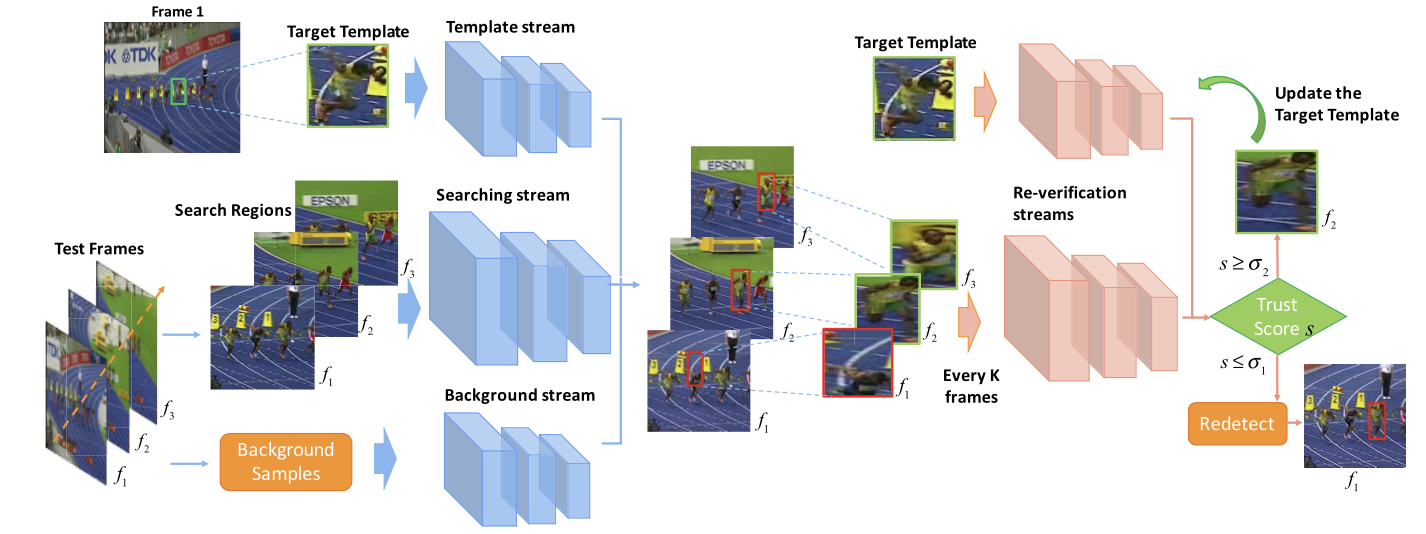
\includegraphics[width = \linewidth]{images/paper8/EMDSLT.png}
    \centering
    \caption{The framework of EMDSLT proposed method.}
    \label{fig:EMDSLT}
\end{figure}

\subsection{RELATED WORK}
Methods such as generative trackers have been developed for finding positions 
in which to find the best candidate during the tracking process. Good 
results have been achieved by compound trackers \cite{0893551105} \cite{0893551118}. Networks such as 
RNNs \cite{0893551121} can be used to predict possible target positions in each frame. 
However, these types of networks have not yet achieved satisfactory results. 
Some methods instead train a CNN offline while the test is done online. Unfortunately, 
these models are not fast. Other models instead if they fail a first 
time, then they will always fail until the target returns to the search region. 
Methods such as \cite{0893551129} \cite{0893551134} search for the target template in subsequent frames 
in the same position, obtaining better performance than methods based on 
similarity but nevertheless are not robust to distracting elements. The proposed 
method instead takes into account both the background patches and 
the target template patches in order to make comparisons on similarities.

\subsection{METHODS}
\subsubsection{Multi Stream Deep Similarity Learning Networks}
A mulit-stream similarity learning network is used in this paper. In the 
proposed framework there are various data streams (Fig. \ref{fig:EMDSLT}):
\begin{enumerate}
    \item Template Stream: the target template defined in the beginning frame;
    \item Searching Stream: the search region;
    \item Background Stream: background patches that sample around the target 
    in the beginning frame.
\end{enumerate}

\subsubsection{Template-Searching-Background Loss}
Several positive $X^+_i$, negative $X^-_i$ and background $B_{i-1,j}$ patches can be 
generated in an image. Patches are considered positive if they have a small 
cosine distance with the target template $T$, on the contrary, patches will be 
considered negative if they are closer to the background patches within the 
search region $S_i$. The loss-function calculation encourages the distance 
between a positive patch and the background patches to be greater than that 
between the positive patch and the target model.
\begin{equation}
    L(T,\{X_{i,k}\}^N_{k=1}, \{B_{i-1}\}^M_{j=1}) = log(1+e^{l_id_i})
\end{equation}
Where $T$ is the target template, $X_{i,k}$ is the $k-th$ candidate patch $X$ of frame 
$i$, $M$ is the number of background patches and $N$ is the number of candidate 
patches $X_{i,k}$. $d(\cdot)$ is the distance function:
\begin{equation}\label{distanceFunc}
    d_i=\sum^M_{j=1} D(T, X_i) - D(X_i, B_{i-1,j})
\end{equation}
where $D$ is the cosine distance that describe the distance of two image patches 
$X_1$ and $X_2$ and $l_i \in \{+1,-1\}$ is the ground truth label of $X_i$. Since the 
loss function must be calculated for each patch, the shortest distance will 
be chosen based on the values returned by the calculation of the following 
loss-function (\ref{FinalLoss}).
\begin{equation}\label{FinalLoss}
    L(T,\{X_{i,k}\}^N_{k=1}, \{B_{i-1}\}^M_{j=1}) = \sum_{k=1}^NL(T,X_{i,k}, \{B_{i-1,j}\}^M_{j=1})
\end{equation}

\subsubsection{Tracking Method}
Background patches are obtained by sampling around the previous positions 
of frame $i-1$. The background patches that have a high correlation with 
the target template will be definitively chosen. Find these patches first, the 
selected $X_i$ pateches will be the ones that will match the target template and 
discriminate against the background patches. Ultimately, the choice of 
patch $X_i$ comes down to an optimization problem.
\begin{equation}
    X_i = \argmin_{X_{i,k} \in S_i}d(T,X_{i,k}, \{B_{i-1,j}\}^M_{j=1})
\end{equation}
where $d(\cdot)$ is a distance function.

\subsubsection{Tracking With Updating}
As already mentioned, the two important aspects of the framework are to 
update the model and allow self-recovery when it is unable to track the target. 
In order to guarantee these two operations, a confidence assessment of the 
monitoring results must be carried out. The set of patches $X_i$ belonging to 
each frame in $(K = k_1)$, is passed to the part of the network that performs 
the re-verification in order to return the "\emph{Trust Score s}" obtained based on 
the similarity with the target template. This score indicates the confidence 
level of the monitoring and can then be used to identify any errors that can 
be corrected with an update of the target template. When the $s$ score is less 
than a $\sigma_1$ threshold, then a failure has occurred. If a failure occurs, then the 
number of frames $K = k_2$ is set lower and then re-detection is performed, 
which would return a new patch $X'_i$, calculated with the formula \ref{newX}, and a 
new score $s'$. If $s'> \sigma_1$, then the new tracking patch will be $X'_i$. In \ref{newX}, $m$ 
represents the matching function, $m(a,b)=f(a)^Tf(b)$, used to obtain 
the Trust Score. If $s$ is greater than $\sigma_2$, then the target template $T$ is updated 
with patches $X_i$.
\begin{equation}\label{newX}
    X'_i = \argmax_{X_{i,k} \in S_i}m(T,X_{i,k})
\end{equation}

\subsection{EXPERIMENTS}
\subsubsection{Network Architecture}
The proposed CNN network is similar to that of AlexNet \cite{0893551108} with five convolutional 
layers of which only the first two are followed by two max pool 
layers. The batch normalization \cite{0893551138} and the ReLu layers are present after 
each convolutional layer except the last.

\subsubsection{Training Details}
To train the model, the videos contained in the ImageNet dataset were used, 
more precisely 90\% of the videos are used as a training set and the remaining 
10\% as a validation set. The training cycles are 240K with mini-batch size 8. 
The target template is set in each random frame of each training video. From 
two other random adjacent frames, the background patches and the search 
region are chosen. In the search region, a candidate patch $Xi$ is labeled 
positive if its overlap with the ground truth bounding box is greater than 
0.7, otherwise it is considered negative. As for the background patches, these 
are selected if they have an overlap with the ground truth in the range 0.1 to 
0.5. The number of frames $k_1$ is set to 10, while $k_2$ is equal to 1 (it 
indicates the re-detection process will take place in sequence on each single 
patch that has caused the tracking to fail), while the $\sigma_1$ and $\sigma_2$ thresholds 
are set accordingly to 1.6 and 2.

\subsubsection{Experimental Setup}
The experiments were conducted on four different types of datasets: OTB-2013 
\cite{0893551142}, OTB-100 \cite{0893551143}, VOT-2015 \cite{0893551144} and VOT-2016 \cite{0893551140}. The first two contain 
a total of 150 bounding-box annotated videos and two metrics, precision 
plots and success plots were used to assess the quality of the tracing. The 
first metric reaches a high value when the distance between the bounding-box 
(ground-truth) centers and the predicted one are less than a certain threshold, 
while the second metric takes into account the overlap of the two components, 
which is calculated with \emph{IoU} index. The last two datasets contain 
a total of 100 videos and the metrics to evaluate the tracking are accuracy, 
robustness and the expected average overlap (\emph{EAO}). To be considered good, 
a tracker must achieve high accuracy and a high AEO score, while it must 
achieve a low robustness score.

\subsubsection{Result and Analysis}
\begin{enumerate}
    \item \emph{Comparison with Recent Real-Time Trackers}: the performance of each tracker, including the one proposed, is shown below. For the OTB dataset, several metrics are used to evaluate its tracking quality. Among these metrics we have those of AUC and precision, while for the VOT dataset the metrics specified above are used (Fig.\ref{fig:PerfComp}).
    \begin{figure}[h!]
        \centering
        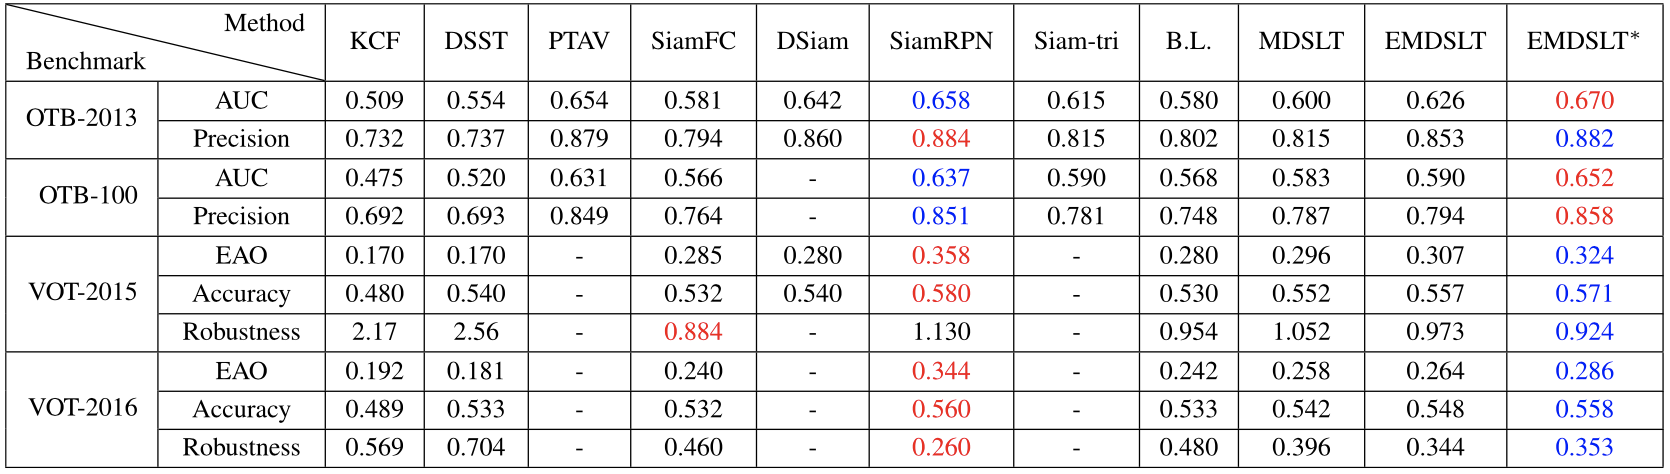
\includegraphics[width = \linewidth]{images/paper8/metrics.png}
        \centering
        \caption{Performance comparison with Recent Real-Time Trackers}
        \label{fig:PerfComp}
    \end{figure}
    \item \emph{Attribute-Based Evaluation}: the presence of distracting elements leads 
    many methods to fail to track them. In figure \ref{fig:AUCScore} it is possible to see the 
    comparison, in terms of AUC score, reached by different methods on 
    the OTB-2013 dataset, when these elements are present. The values 
    in red are the highest and are obtained from the best method, while 
    those in blue are placed in second position.
    \begin{figure}[h!]
        \centering
        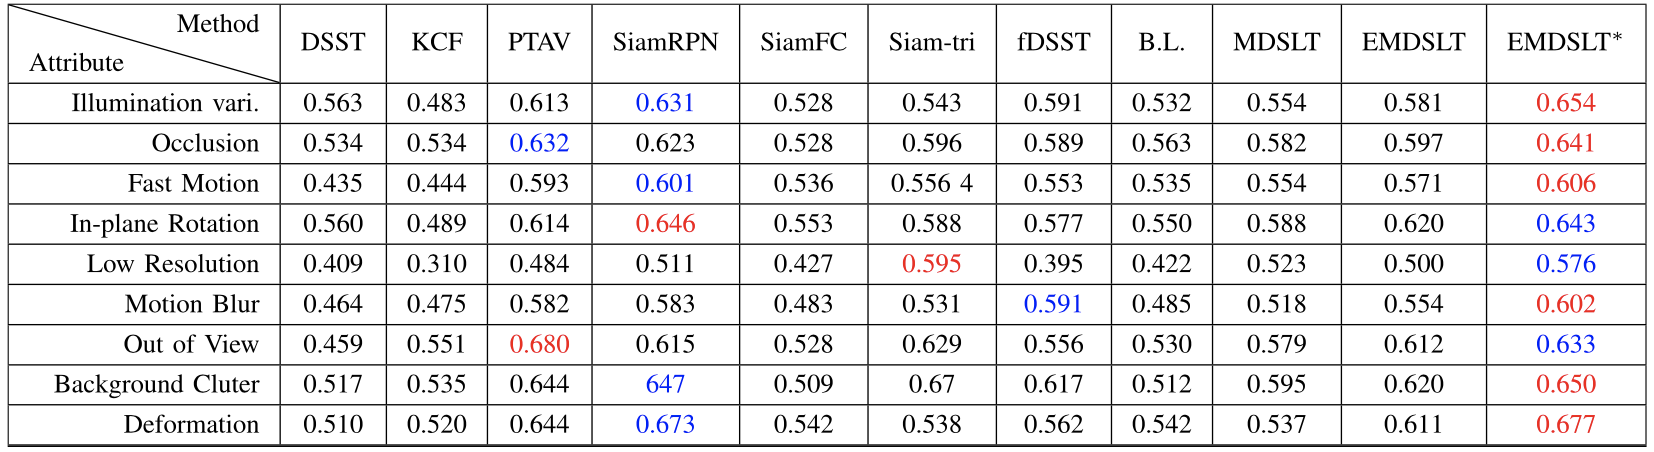
\includegraphics[width = \linewidth]{images/paper8/AUC.png}
        \centering
        \caption{AUC score on OTB-2013 dataset.}
        \label{fig:AUCScore}
    \end{figure}
    \item \emph{Qualitative Evaluation}: The use of the Template-Searching-Background 
    (TSB), allows you to use the background patches to train the model 
    (Fig.\ref{fig:TSBMin}). This method helps to minimize the relative distance $d(\cdot)$ (\ref{distanceFunc}) 
    which translated into other words means bringing the target template 
    closer to the $X_i^+$ samples and at the same time moving the background 
    distractors $B_i$ away from the positive sample. This method allows for 
    better performance than existing state-of-the-art models. A visual example 
    of comparison of the trackers made by the different methods, 
    including the one proposed, is visible in figure \ref{fig:qualitativeTracking}.
    \begin{figure}[h!]
        \centering
        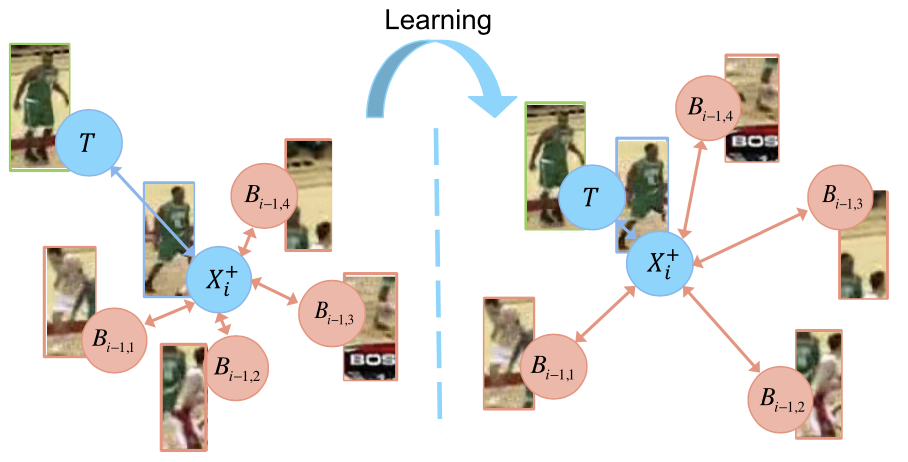
\includegraphics[width = \linewidth]{images/paper8/TSB.png}
        \centering
        \caption{Template-Searching-Background to minimizes the relative distance.}
        \label{fig:TSBMin}
    \end{figure}
    \begin{figure}[h!]
        \centering
        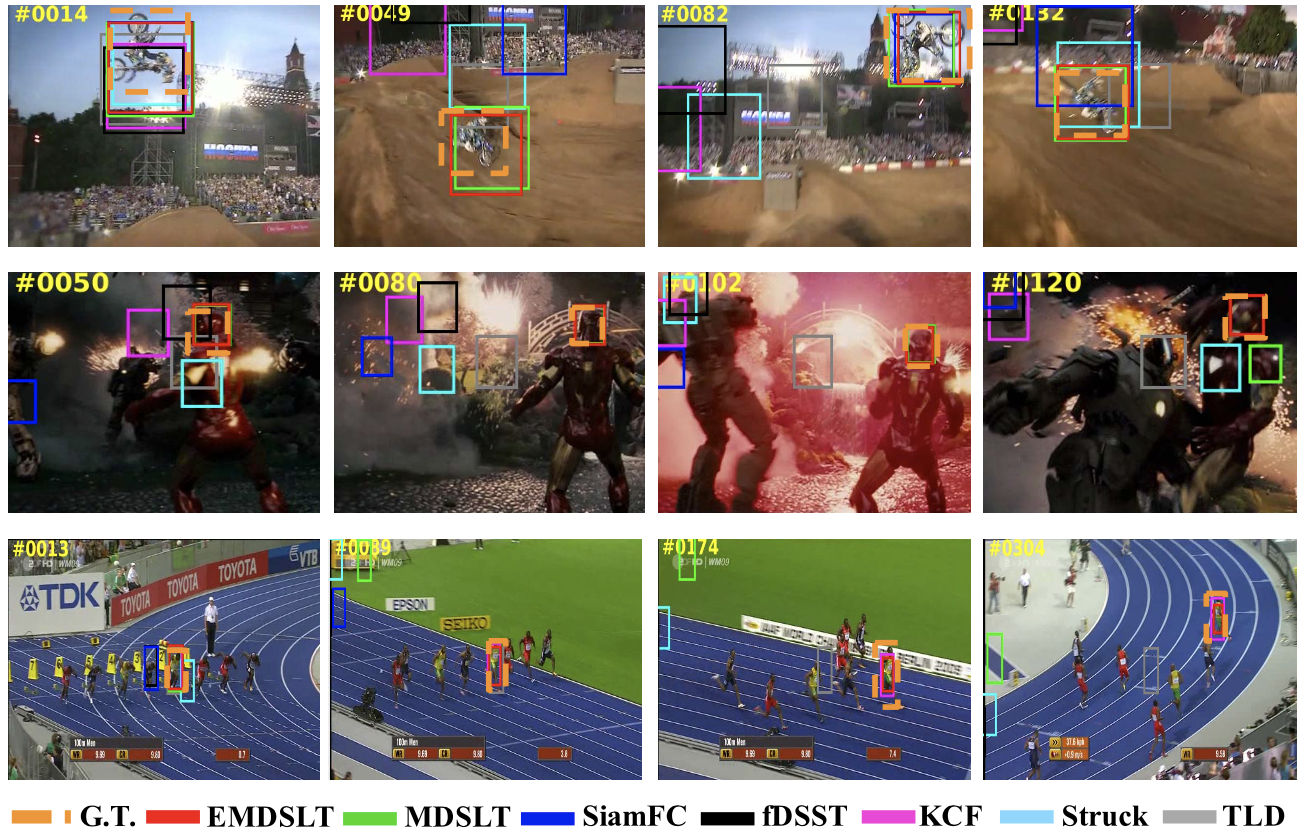
\includegraphics[width = \linewidth]{images/paper8/qualitative.png}
        \centering
        \caption{Qualitative reuslt of seven trackers. The bounding box with an orange dotted line shows the ground-truth localization of the target object.}
        \label{fig:qualitativeTracking}
    \end{figure}
\end{enumerate}

\subsection{CONCLUSION}
The proposed framework, from the results obtained in the benchmarks, seems 
to be the best. The achievement of these results were possible thanks to the 
integration of a verification and detecting method. The use of the TSB 
method was fundamental, which, by reducing the relative distance between 
the various patches, allowed for good model learning.